The weight counter system is made with 5 different source files responsible for different parts. 
These can be seen in \cref{fig:architecture}. 
The parts are \mintinline{c}{Menu}, \mintinline{c}{TFT Driver}, \mintinline{c}{Keypad}, \mintinline{c}{Weight Counter} and \mintinline{c}{ADC}.
The menu system is called from the \mintinline{c}{main} and is responsible for the different actions of the system. 
The \mintinline{c}{Menu} system calls the state function depending on which state the menu is in. 
Then it calls the \mintinline{c}{menuStatefunc} depending on the input from the \mintinline{c}{Keypad}. The functions \mintinline{c}{getLetter} and \mintinline{c}{getNumber} is used when the user needs to enter a letter and number respectively. 
The menu system uses the \mintinline{c}{TFT Driver} to output information to the display using the \mintinline{c}{write} and \mintinline{c}{ClearArea} functions. 
The menu system uses the keypad function \mintinline{c}{NumKeyScan} to get the input from user.  
The menu uses \mintinline{c}{Weight Counter} function \mintinline{c}{Counter} when the weight cell is used as a weight counter. 
The \mintinline{c}{ADC_single_avg} is called from \mintinline{c}{Menu} when the user wants to add a new item to the weight counter. 
The function then measures the weight of the item.

\begin{figure}
\centering
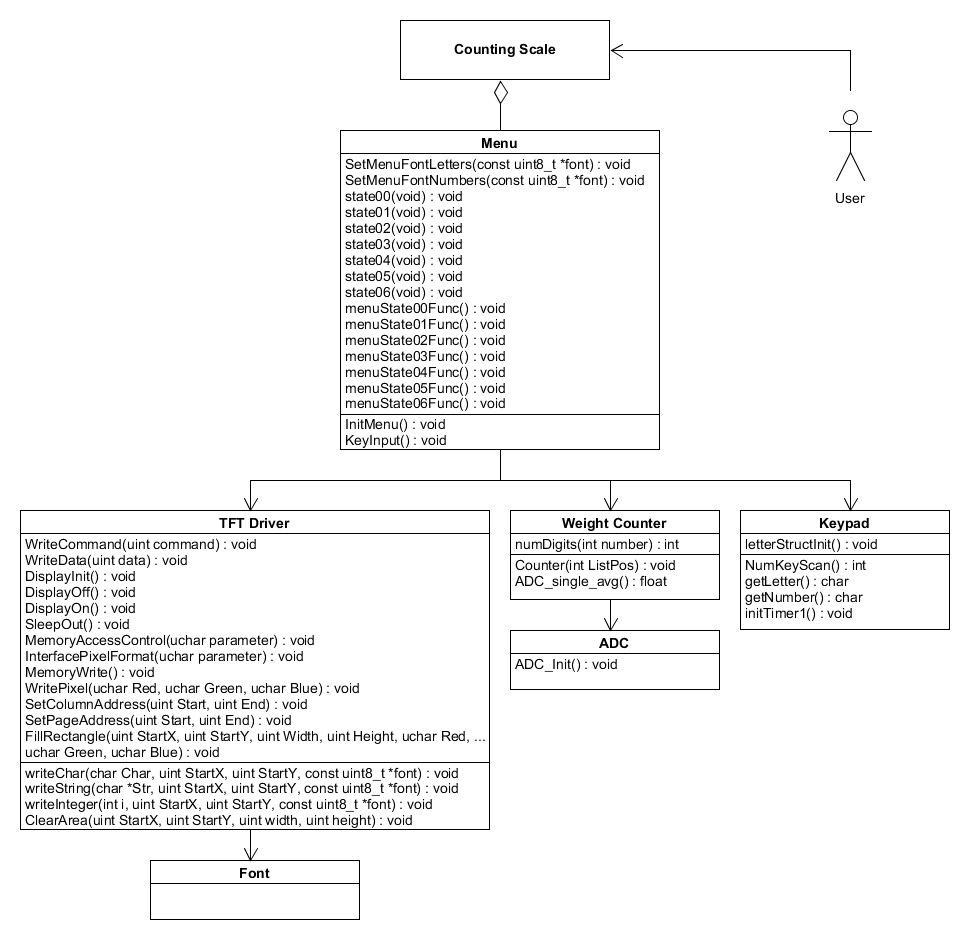
\includegraphics[width=1\linewidth]{graphics/architecture}
\caption{Software architecture of the Counting Scale system. Functions below the line are used in other source files while functions above the line are only used in their own respective sourcefile.}
\label{fig:architecture}
\end{figure}
